\documentclass[12pt, twoside]{article}
\documentclass[12pt, twoside]{article}
\usepackage[letterpaper, margin=1in, headsep=0.2in]{geometry}
\setlength{\headheight}{0.6in}
%\usepackage[english]{babel}
\usepackage[utf8]{inputenc}
\usepackage{microtype}
\usepackage{amsmath}
\usepackage{amssymb}
%\usepackage{amsfonts}
\usepackage{siunitx} %units in math. eg 20\milli\meter
\usepackage{yhmath} % for arcs, overparenth command
\usepackage{tikz} %graphics
\usetikzlibrary{quotes, angles}
\usepackage{graphicx} %consider setting \graphicspath{{images/}}
\usepackage{parskip} %no paragraph indent
\usepackage{enumitem}
\usepackage{multicol}
\usepackage{venndiagram}

\usepackage{fancyhdr}
\pagestyle{fancy}
\fancyhf{}
\renewcommand{\headrulewidth}{0pt} % disable the underline of the header
\raggedbottom
\hfuzz=2mm %suppresses overfull box warnings

\usepackage{hyperref}
\usepackage{float}

\title{Algebra 2}
\author{Chris Huson}
\date{September 2024}

\fancyhead[LE]{\thepage}
\fancyhead[RO]{\thepage \\ First and last name: \hspace{2.5cm} \,\\ Section: \hspace{2.5cm} \,}
\fancyhead[LO]{BECA/Huson/Precalculus: Sequences \\* 17 September 2024}

\begin{document}
\subsubsection*{1.10 Pretest: Powers and radicals, sequences \hfill Mental math - no calculators}
\begin{enumerate}[itemsep=0.5cm]

\item Memorize the squares to 100. \hfill \emph{3.OA.7 Fluently multiply and divide within 100}
    \begin{multicols}{2}
        \begin{enumerate}[itemsep=0.5cm]
            \item $8^2 =$
            \item $2^2 =$
            \item $5^2 =$
            \item $4^3 =$
        \end{enumerate}
    \end{multicols}

\item Memorize the square roots of whole numbers through 100 and cubes through five.
    \begin{multicols}{2}
        \begin{enumerate}[itemsep=0.5cm]
            \item $\sqrt{9} =$
            \item $\sqrt{47} =$
            \item $\sqrt{64} =$
            \item $\sqrt{36} =$
            \item $\sqrt[3]{8} =$
            \item $\sqrt[3]{27} =$
          \end{enumerate}
    \end{multicols}

\item Round to the \emph{nearest thousandth}.
  \begin{multicols}{2}
  \begin{enumerate}[itemsep=1.5cm]
    \item $A=105.194547$
    \item $V=59.10811$
  \end{enumerate}
  \end{multicols} \vspace{0.5cm}

\item Simplify each expression by ``collecting like terms''
\begin{enumerate}[itemsep=2cm]
  \begin{multicols}{2}
    \item $3x+4x^2-5x+11x^2$
    \item $12y+2\sqrt{11}-7y-4\sqrt{11}$
  \end{multicols}
  \end{enumerate} \vspace{1cm}

\item Use the function $f(x) = -4x+8$ to answer the questions.
  \begin{multicols}{2}
  \begin{enumerate}[itemsep=2cm]
      \item What is $f(0)$?
      \item Find $f(\frac{1}{4})$
      \item Solve for $x$ if $f(x) = 20$.
  \end{enumerate}
  \end{multicols} \vspace{1cm}

\newpage

% June 2019 Regents - Problem 8
\item Which sequence is defined recursively?
\begin{enumerate}
    \item $a_n = 3n + 1$
    \item $a_1 = 2$ and $a_{n+1} = a_n + 3$
    \item $a_n = 4n - 5$
    \item $a_n = 2^n$
\end{enumerate}

% June 2019 Regents - Problem 19
\item The first term of a sequence is $a_1 = 7$ and each subsequent term is found by adding 5 to the previous term. Which formula represents the $n$th term of the sequence?
\begin{enumerate}
    \item $a_n = 5n + 2$
    \item $a_n = 5n + 7$
    \item $a_n = 5n - 3$
    \item $a_n = 7n + 5$
\end{enumerate}

\item Which of the following is the recursive formula for the sequence $40, 30, 22.5, \ldots$
  \begin{multicols}{2}
  \begin{enumerate}
    \item $g_n = 40 \left( \frac{3}{4} \right)^n$
    \item $g_1 = 40$ \\ $g_n = g_{n-1} -10$
    \item $g_n = 40 \left( \frac{3}{4} \right)^{n-1}$
    \item $g_1 = 40$ \\ $g_n = \frac{3}{4} g_{n-1}$
  \end{enumerate}
  \end{multicols}

% January 2019 Regents - Problem 16
\item A sequence is defined recursively by $ a_1 = 2 $ and $ a_{n+1} = 3a_n + 1 $ for $ n \geq 1 $. Find the first four terms of the sequence. \vspace{2cm}

% Example Problem 2
\item Given the arithmetic sequence where $ a_1 = 5 $ and the common difference $ d = 3 $, write an explicit formula for the $n$th term of the sequence. What is the 10th term?

% Example Problem 3
%\item A geometric sequence has a first term of \( a_1 = 4 \) and a common ratio of \( r = \frac{1}{2} \). Write the recursive formula for the sequence. Calculate the 6th term.

\newpage
\item Write a recursive formula for the sequence $5, 10, 15, 20, \dots$ \vspace{2cm}


% January 2019 Regents - Problem 16
\item Savannah just got contact lenses. Her doctor said she can wear them 2 hours the first day, and can then increase the length of time by 30 minutes each day. If this pattern continues, which formula would not be appropriate to determine the length of time, in either minutes or hours, she could wear her contact lenses on the nth day?
\begin{enumerate}
    \item $t_n = 120 + 30(n-1)$
    \item $t_n = 2 + 0.5(n-1)$
    \item $t_n = 2 + 30n$
    \item $t_n = 120 + 0.5(n-1)$
\end{enumerate}

\item A sequence $f(n)$ is shown below as a graph and as a table.
\begin{enumerate}
  \begin{multicols}{2}
  \item  Is sequence geometric or arithmetic? \\Explain how you know. \par \vspace{2cm}
  \begin{tabular}{c|c}
    $n$ & $f(n)$ \\ \hline
    0 & 16 \\ 
    1 & 8 \\ 
    2 & 4 \\ 
    3 & 2 \\ 
    4 & 1 \\ 
    \end{tabular} \vspace{1cm}
    \begin{center}
      \begin{tikzpicture}[yscale=0.4]
          \draw [thin, color=lightgray, xstep=0.5cm,ystep=2.0cm] (0,0) grid (5,18);
          \foreach \x in {0,1,2,...,5}
          \draw (\x cm,3pt) -- (\x cm,-3pt) node[below] {$\x$};
          \foreach \y in {0,2,...,18}
          \draw[shift={(0,\y)},color=black] (2pt,0pt) -- (-2pt,0pt) node[left]  {$\y$};
          \draw [thick, ->] (0,0) -- (+5.4,0) node [above right] {$n$};
          \draw [thick, ->] (0,0) -- (0,18.8) node [right] {$f(n)$};
          \node at (0,16){$\bullet$};
          \node at (1,8){$\bullet$};
          \node at (2,4){$\bullet$};
          \node at (3,2){$\bullet$};
          \node at (4,1){$\bullet$};
          %\draw [thick, <->,smooth,domain=-0.5:8.5] plot(\x,-\x*\x+8*\x);
      \end{tikzpicture}
      \end{center}
    \end{multicols}
        \item Write the recursive formula for the sequence. \vspace{3cm}
    \end{enumerate}

\end{enumerate}
\end{document}
